\documentclass{beamer}


\mode<presentation> {
  \usetheme{Warsaw}
  % ou autre ...

  \setbeamercovered{transparent}
}


\usepackage[french]{babel}
% or autre comme par exemple \usepackage[english]{babel}

\usepackage[latin1]{inputenc}
% or autre

\usepackage{times}
\usepackage[T1]{fontenc}
\usepackage{graphicx}

\title[Titre court] 
{MY TWIN}

\subtitle {Mi otro Yo}

\author[] 
{Developers: \\Hernan Ullon\inst{1} \and Kevin Calderon\inst{2}  \and Cesar San Lucas\inst{3}}


\AtBeginSubsection[] {
  \begin{frame}<beamer>{DESCRIPCION}
    \tableofcontents[currentsection,currentsubsection]
  \end{frame}
}


\begin{document}



\begin{frame}

\center

\includegraphics[scale=0.3]{logo.jpg}
  \titlepage


\end{frame}

\begin{frame}{DESCRIPCION}
  \tableofcontents
\end{frame}


\section{IDEA}

\subsection{Problematica}

\begin{frame}{Problematica}{Ideas:\\Simples\\Dificiles\\Sencillas\\\\Ninguna Convencia}

\center
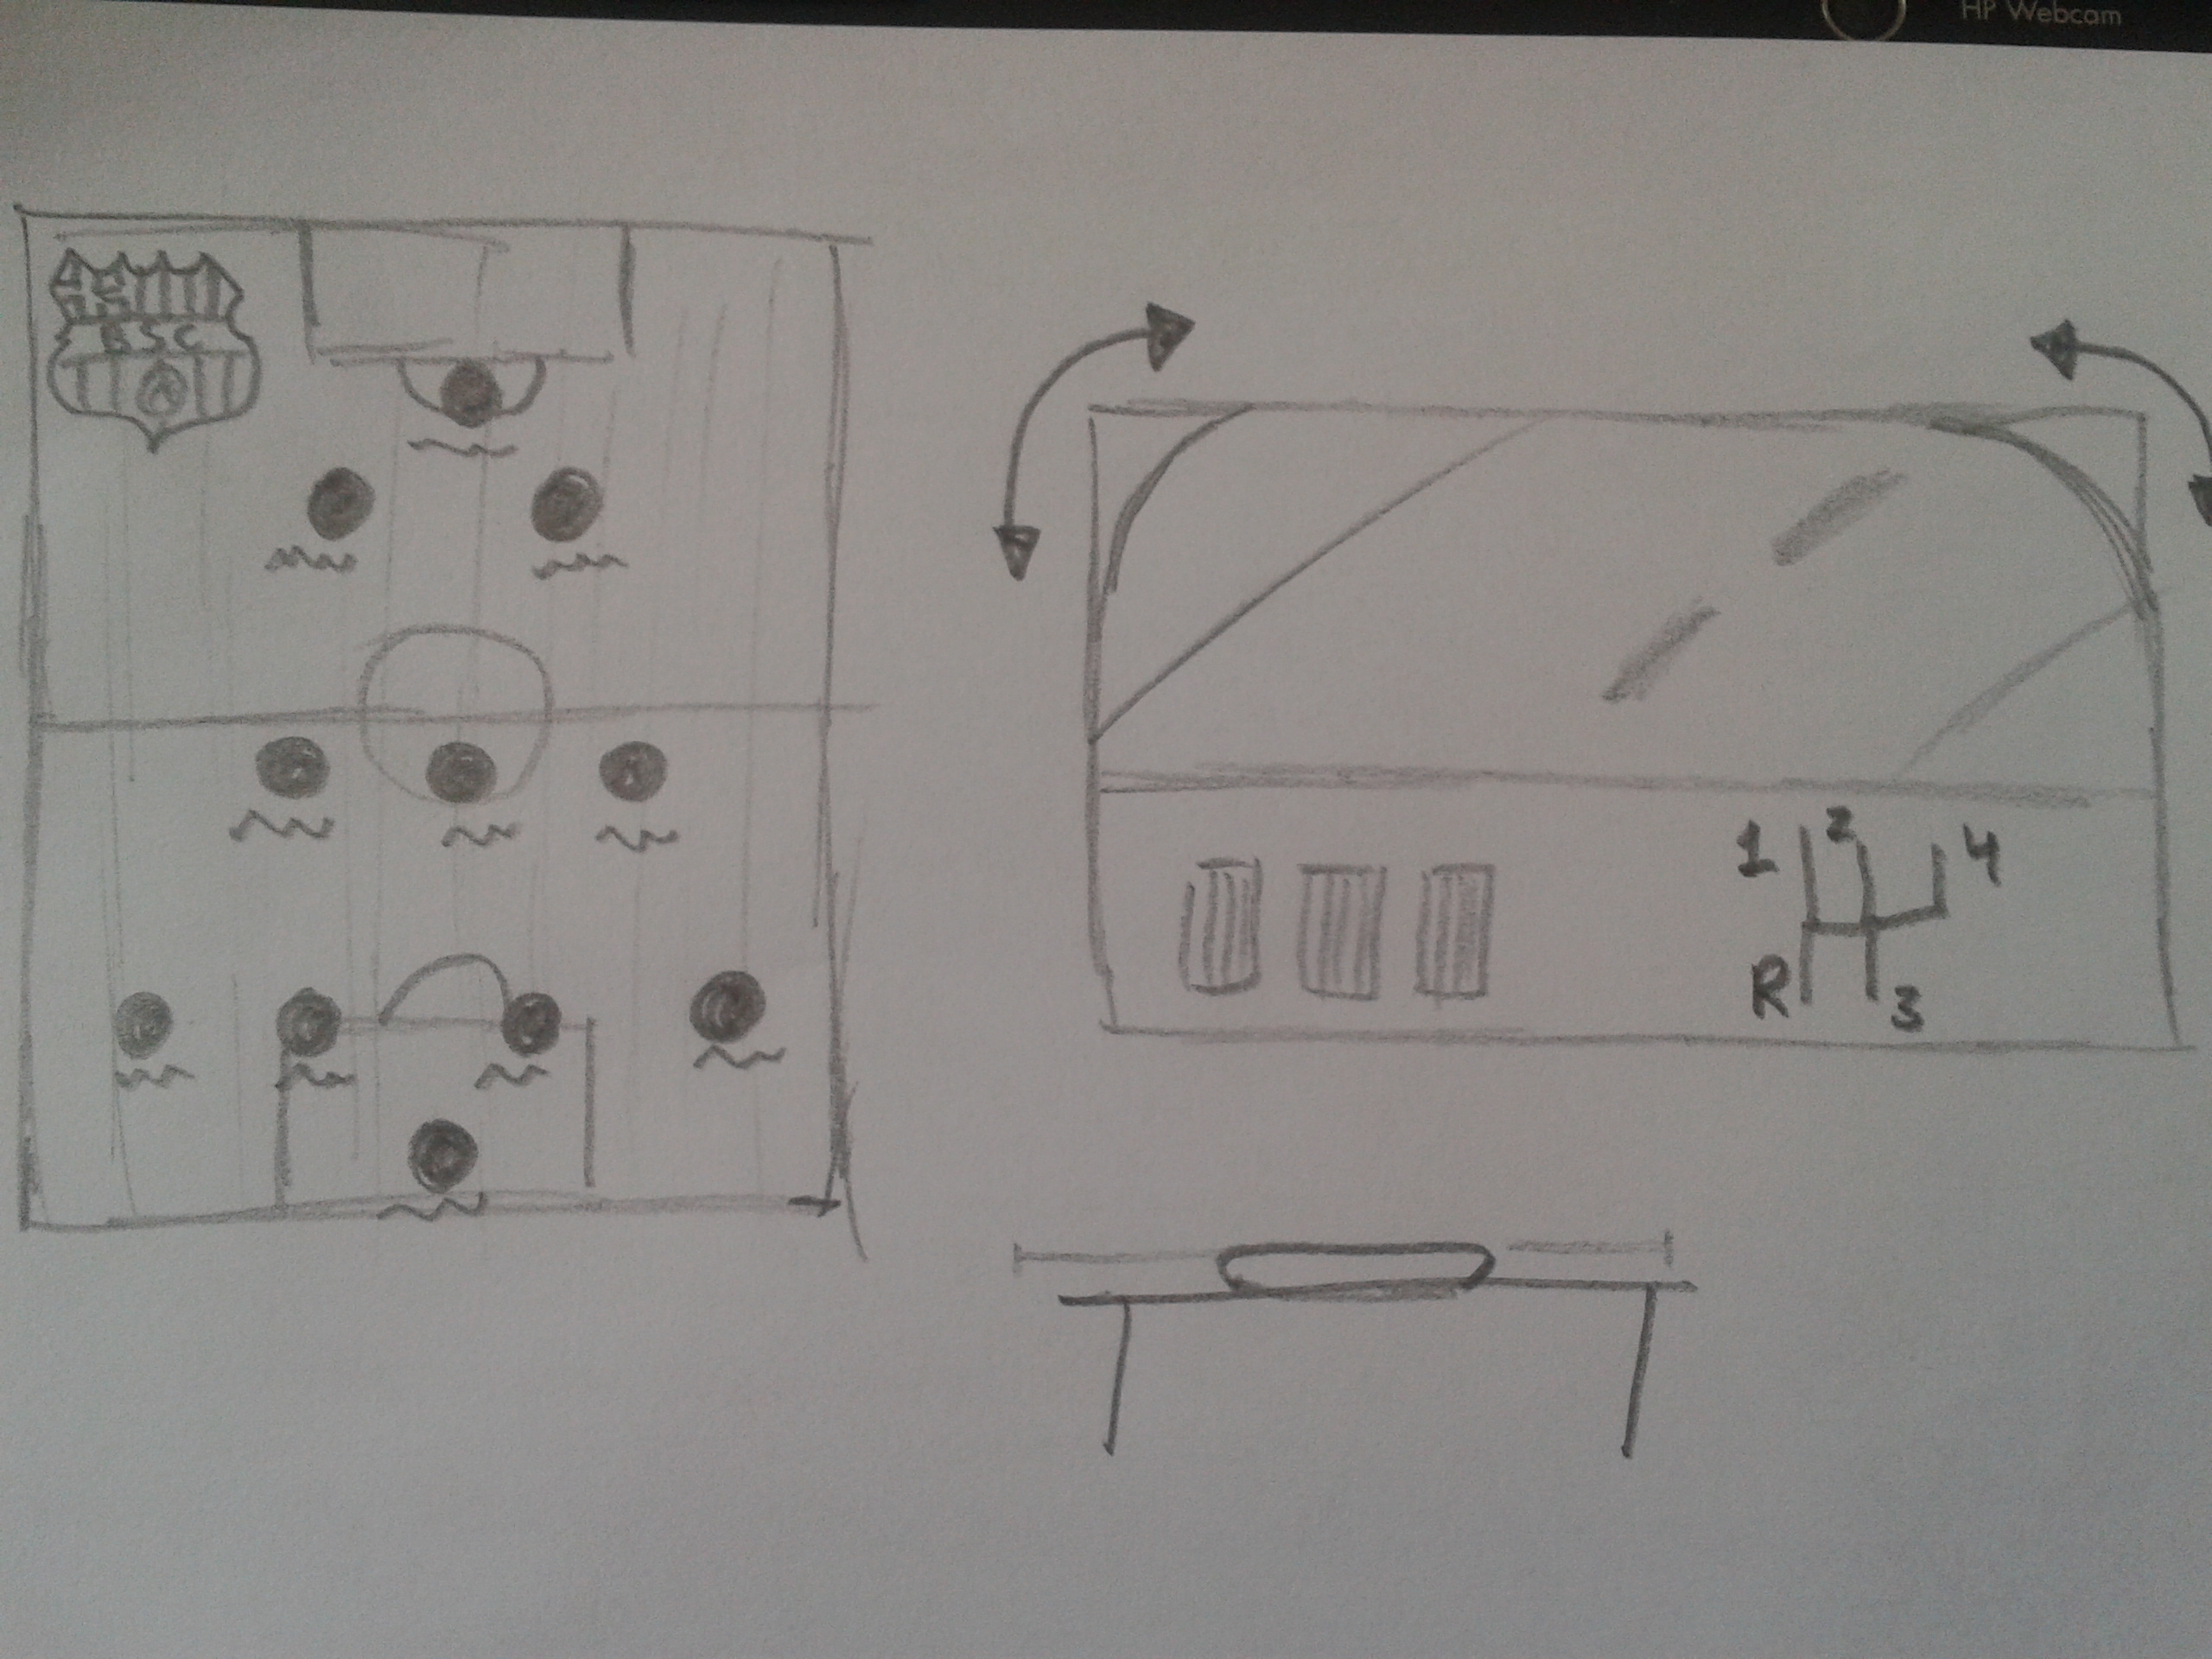
\includegraphics[scale=0.07]{problematica.jpg}


\end{frame}

\subsection{Idea Final}

\begin{frame}{Idea Final}
\center
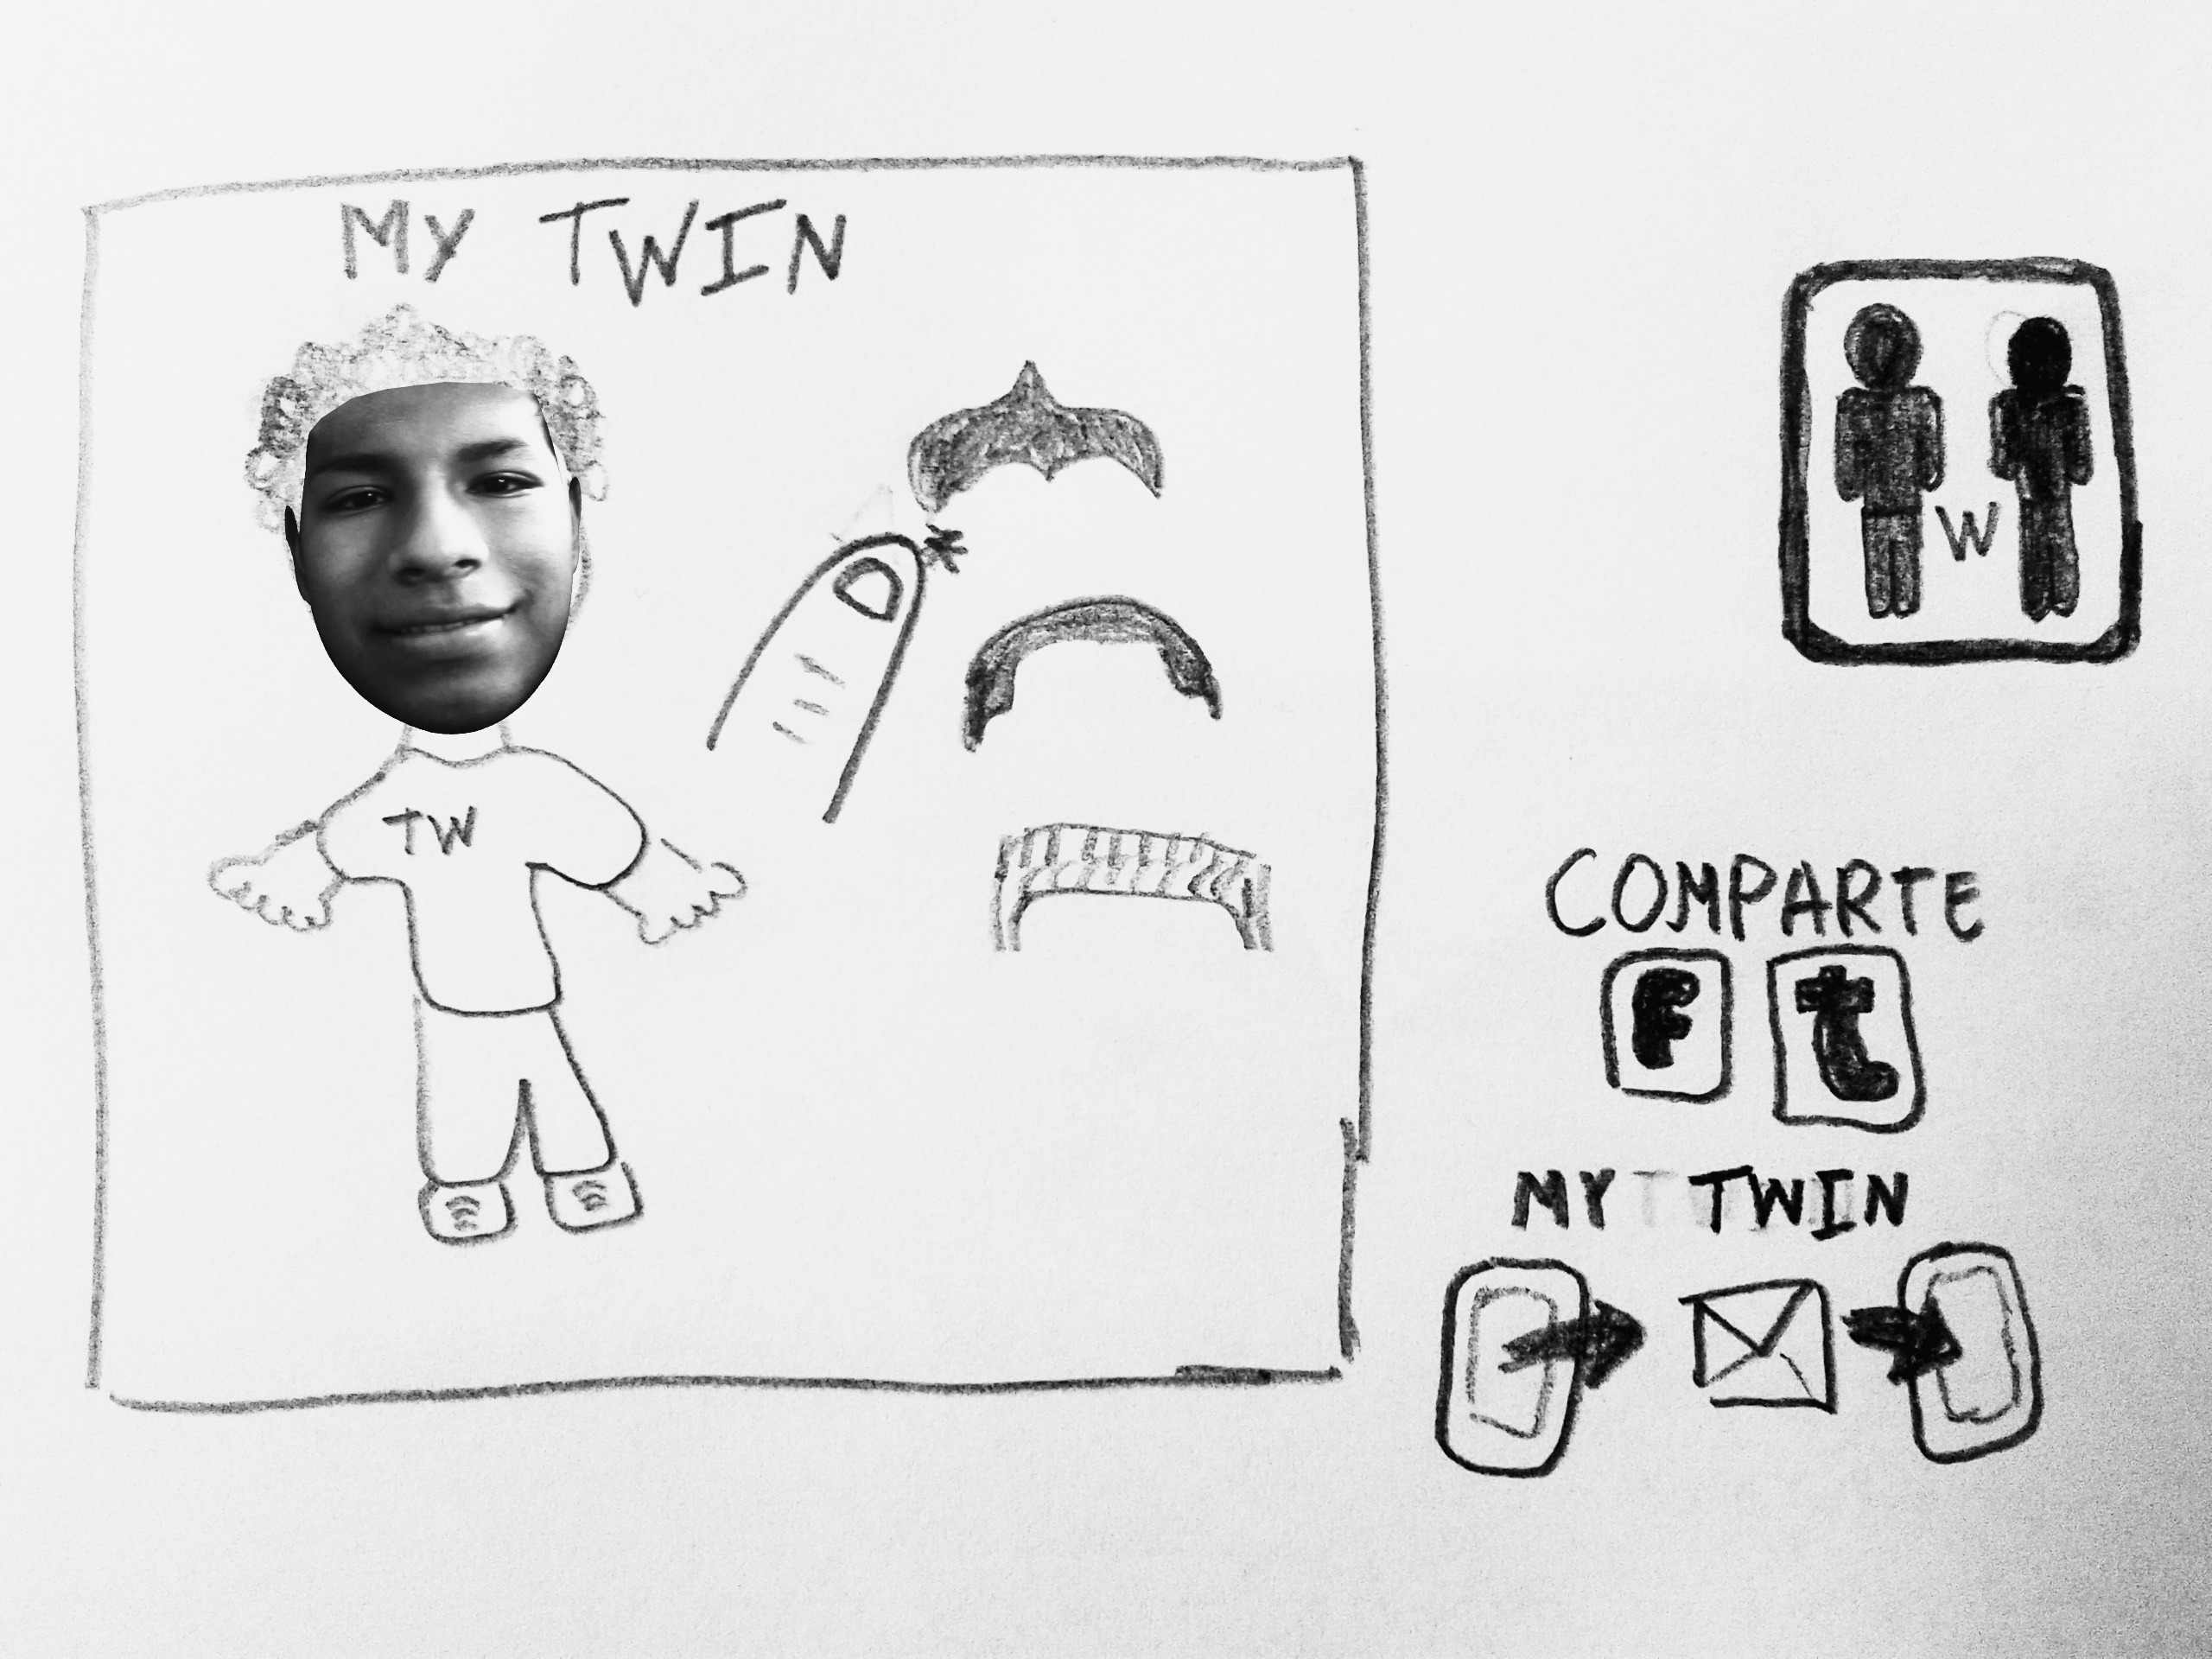
\includegraphics[scale=0.09]{idea.jpg}

\end{frame}




\section{MY TWIN}

\subsection{Descripcion}

\begin{frame}{Descripcion}{DIVERTIDA}
   
\includegraphics[scale=0.5]{442.jpg}
\end{frame}

\begin{frame}{Descripcion}{REALISTA}
   
\includegraphics[scale=0.5]{droid.jpg}
\end{frame}

\begin{frame}{Descripcion}{SOCIAL}
   
\includegraphics[scale=0.5]{fb.jpg}
\end{frame}




\subsection{Recursos}

\begin{frame}{RECURSOS}{CAMARA}
   
\includegraphics[scale=0.5]{camara.jpeg}
\end{frame}

\begin{frame}{RECURSOS}{ACELEROMETRO}
   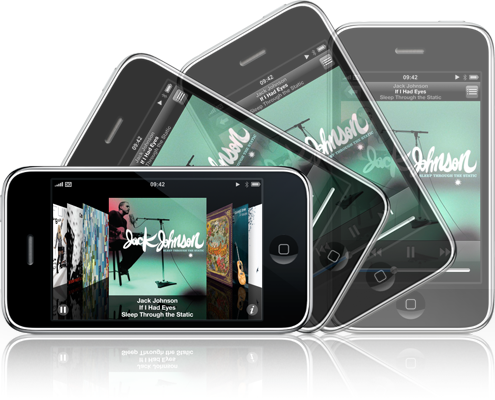
\includegraphics[scale=0.5]{acelerometro.png}
\end{frame}

\begin{frame}{RECURSOS}{MICROFONO}
   
\includegraphics[scale=0.5]{voice.jpg}
\end{frame}





\appendix
\section<presentation>*{\appendixname}
\subsection<presentation>*{Lectures complémentaires}

\begin{frame}[allowframebreaks]
  \frametitle<presentation>{Lectures complémentaires}

  \begin{thebibliography}{10}

  \beamertemplatebookbibitems

  \bibitem{Auteur1990}
    A.~Auteur.
    \newblock {\em Livre de quelque chose}.
    \newblock Une Edition, 1990.


  \beamertemplatearticlebibitems

  \bibitem{Quelqu'un2000}
    S.~Quelqu'un.
    \newblock Et ceci et cela.
    \newblock {\em Journal de ceci et cela}, 2(1):50--100,
    2000.
  \end{thebibliography}
\end{frame}

\end{document}